\begin{minipage}{0.65\textwidth}
    \vspace{-1mm}

    \begin{figure}[h]
        \centering
        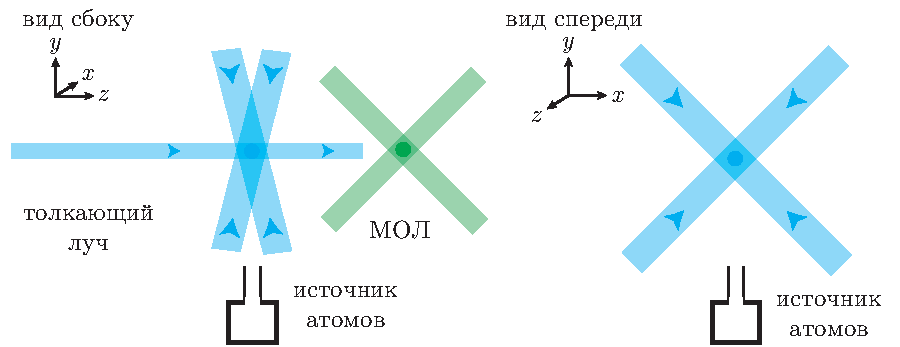
\includegraphics[width=0.9\textwidth]{../MOT/figs/2dmot_v3.pdf}
        \vspace{1mm}
        \caption{Принципиальная схема лучей 2D-МОЛ}
        \label{fig:2dmots}
    \end{figure}

    \vspace{-8mm}

    \begin{figure}[h]
        \centering
        \includegraphics[width=1.0\textwidth]{../MOT/figs/vcap2d_delta-Ds.png}
        \caption{Зависимость скорости захвата 2D-МОЛ для различных мощностей от отстройки $\delta$ лучей 2D-МОЛ и размера $D$ пучков}
    \end{figure}
\end{minipage}
\hfill
\begin{minipage}{0.31\textwidth}

Загрузка МОЛ: \vspace{-3mm}
\begin{align*}
    % \sub{\Phi}{load} &\propto \sub{\Phi}{tot} \int_{0}^{\vcap} v^3 e^{-v^2/\alpha^2} \d v \\
    \sub{\Phi}{load} &\propto  \sub{\Phi}{sol} \left(\frac{\sub{v}{\textcolor{blue}{cap}}}{\alpha}\right)^4
\end{align*}


Скорости захвата: \vspace{-3mm}
\begin{equation*}
    m \int_{\vcap}^{0} \frac{v}{F(v)} \d v = D
\end{equation*}


Критическое расстояние: \vspace{-3mm}
\begin{equation*}
    \sub{l}{крит} \sim \sqrt{\frac{\sub{h}{крит} \sub{v}{\textcolor{green}{cap}}^2}{g}} \sim 1\,\text{м}
\end{equation*}


\phantom{42}

При $T \sim 700 \dC$: \\ 
$\sub{\Phi}{load}(\sub{v}{\textcolor{blue}{cap}} = 40\,\text{м/c}) \sim 10^8\,\text{c}^{-1}$

\end{minipage}